\documentclass[xetex,mathsans,sans,aspectratio=169]{beamer}
\usepackage{listings}
\usetheme{Boadilla}
\usecolortheme{orchid}
\usepackage{fontspec}
\setsansfont{Basis Grotesque}
\setbeamertemplate{navigation symbols}{}
\usepackage{amsmath}
\usepackage{multicol}

% The title slide information about the presenter(s) eg. name(s), role(s)
\newcommand{\presenter}{<presenter name(s), role(s)>}

% The text for the presenter footer eg. first name(s)
\newcommand{\presenterfooter}{<presenter fname(s)>}

% The footer title of the presentation (optional - default is 'NuCypher')
\newcommand{\titlefooter}{NuCypher}

% The email name prefix for the presenter i.e. <email_prefix>@nucypher.com
\newcommand{\emailname}{<email\_prefix>}

% The name of the event
\newcommand{\event}{<event name>}

% The date of the event with format: dd MMM yyyy
\newcommand{\eventdate}{<dd MMM yyyy>}


% Example usage:
%
%     \newcommand{\presenter}{MacLane Wilkison, CEO \& Co-Founder}
%     \newcommand{\presenterfooter}{MacLane}
%     \newcommand{\titlefooter}{NuCypher}
%     \newcommand{\emailname}{maclane}
%     \newcommand{\event}{Eth SF}
%     \newcommand{\eventdate}{05 Oct 2018}
%


\title[\titlefooter]{
\includegraphics[width=5.5cm]{pdf/nucypher_logo.pdf}}
\author[\presenterfooter]{\presenter}
\date[\eventdate]{\event, \eventdate}

\begin{document}
    \begin{frame}
        \titlepage
    \end{frame}

    \begin{frame}
      \frametitle{NuCypher Overview}
        \begin{itemize}
            \item Use cryptography to build the tools \& infrastructure to preserve data privacy
            \item Privacy-preserving solutions for distributed applications
              \begin{itemize}
                  \item Proxy Re-encryption (PRE)
                  \begin{itemize}
                    \item Secure data-sharing and access control of encrypted data
                  \end{itemize}
                  \item Fully Homomorphic Encryption (FHE)
                  \begin{itemize}
                    \item Perform arbitrary operations on encrypted data
                  \end{itemize}
              \end{itemize}
            \item Blockchain \& Private Deployments
        \end{itemize}
    \end{frame}

    \begin{frame}
        \frametitle{Public Key Encryption (PKE)}
        \begin{figure}
            \centering
            \includegraphics<1>[width=11cm]{pdf/pke-multi.pdf}
            \includegraphics<2>[width=11cm]{pdf/pke-multi-hack.pdf}
        \end{figure}

        Limitations
        \begin{itemize}
            \item<2> Decryption required before sharing
            \item<2> Not scalable
            \item<2> Complex access revocation
        \end{itemize}
    \end{frame}

    \begin{frame}
        \frametitle{What is proxy re-encryption (PRE)}
        \begin{figure}
            \centering
            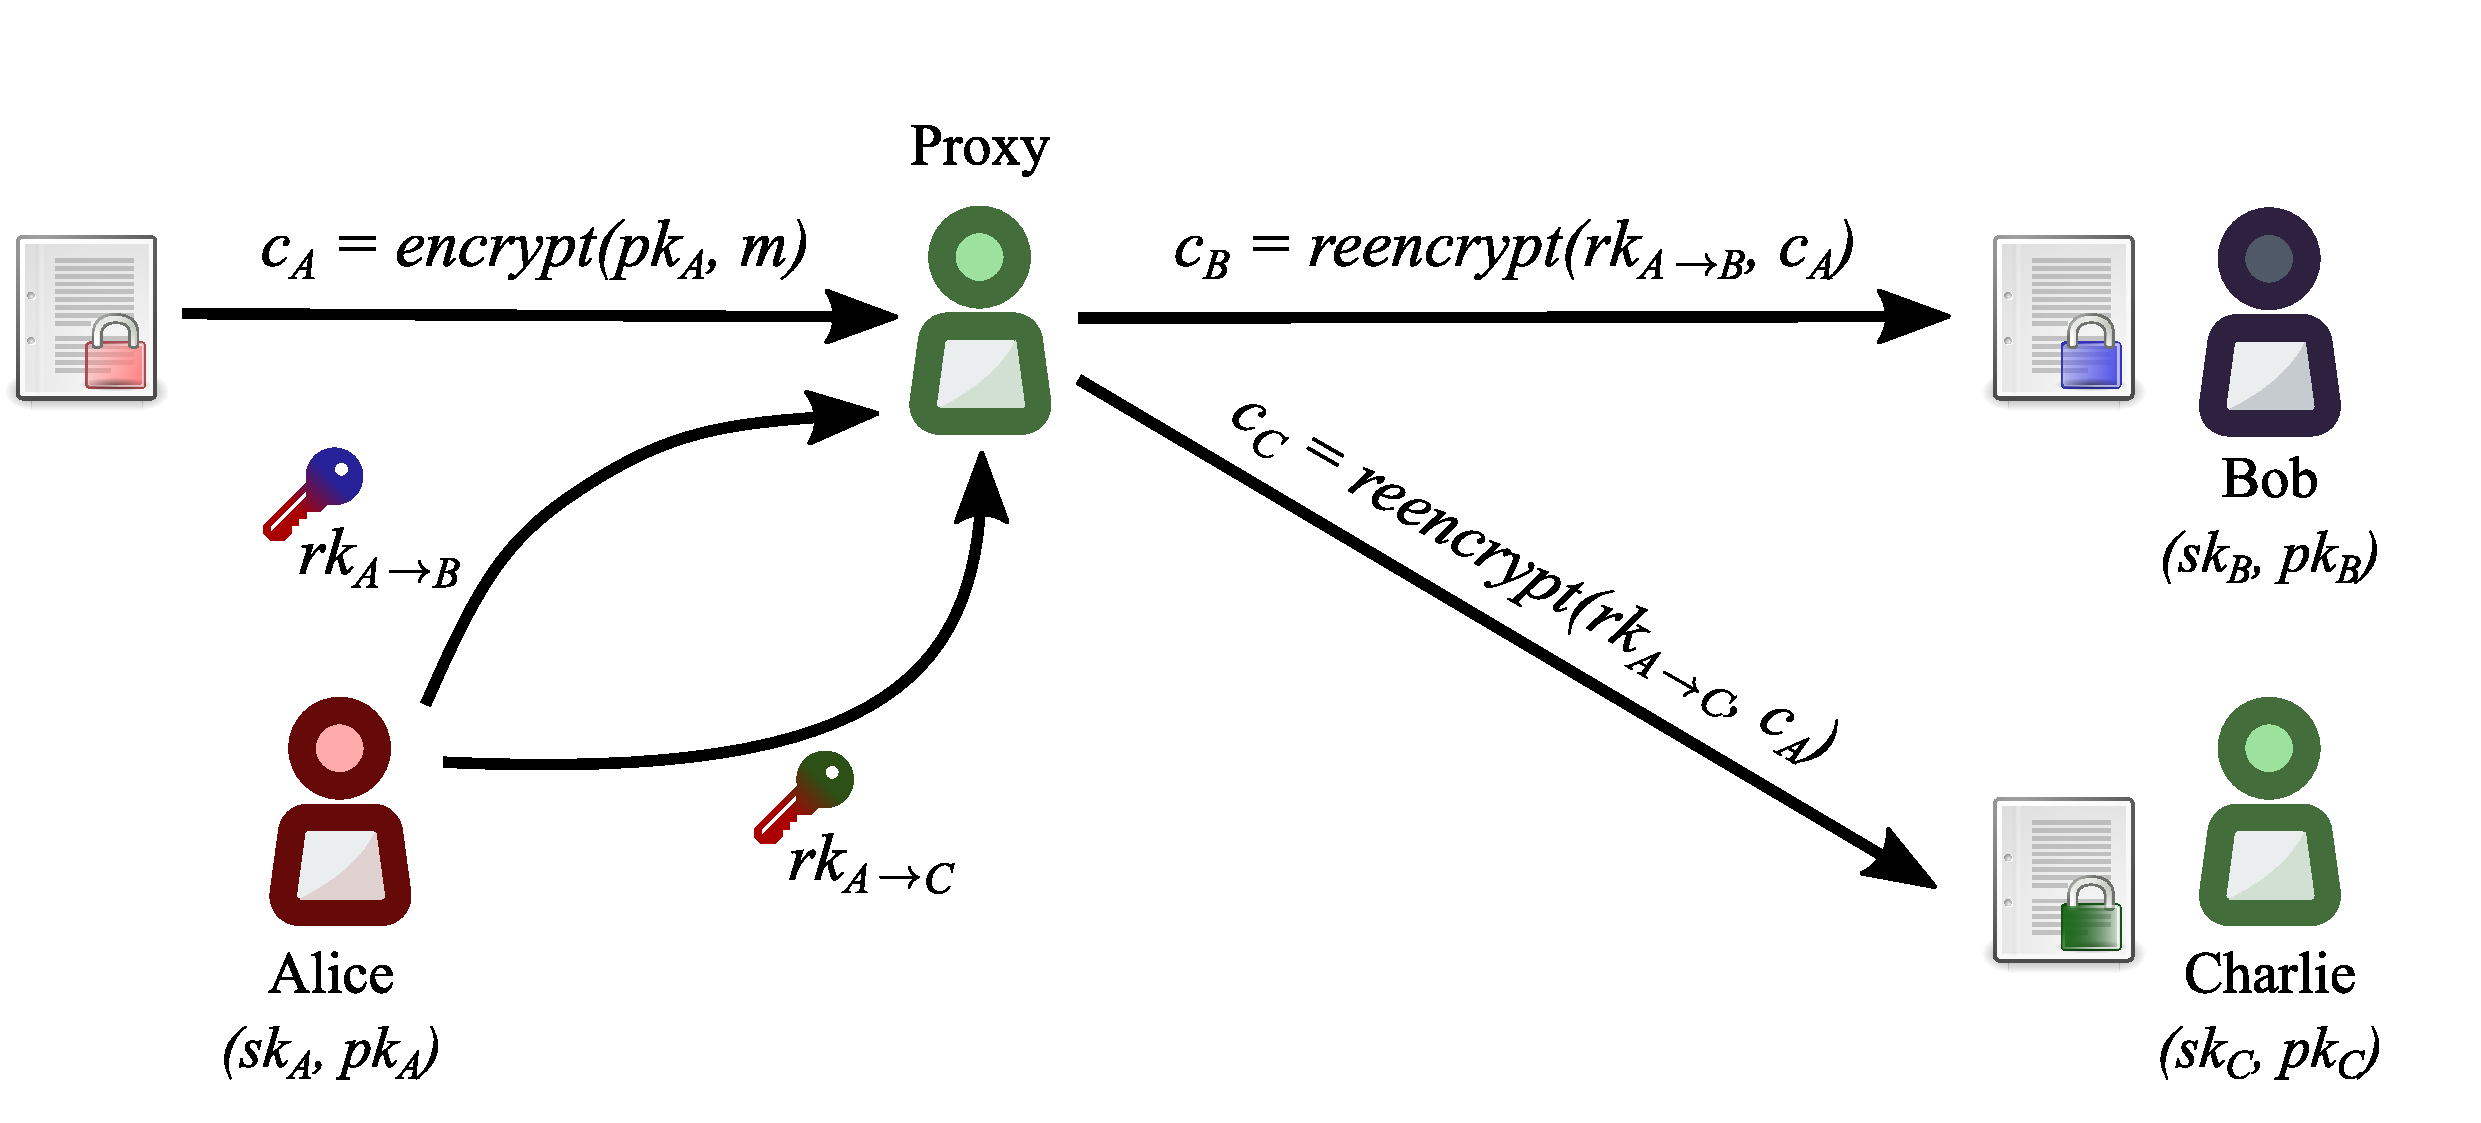
\includegraphics[width=13cm]{pdf/pre-multi.pdf}
        \end{figure}
    \end{frame}

    \begin{frame}
        \frametitle{Solution}
        \framesubtitle{Proxy re-encryption + Key Management}
        \begin{figure}
            \centering
            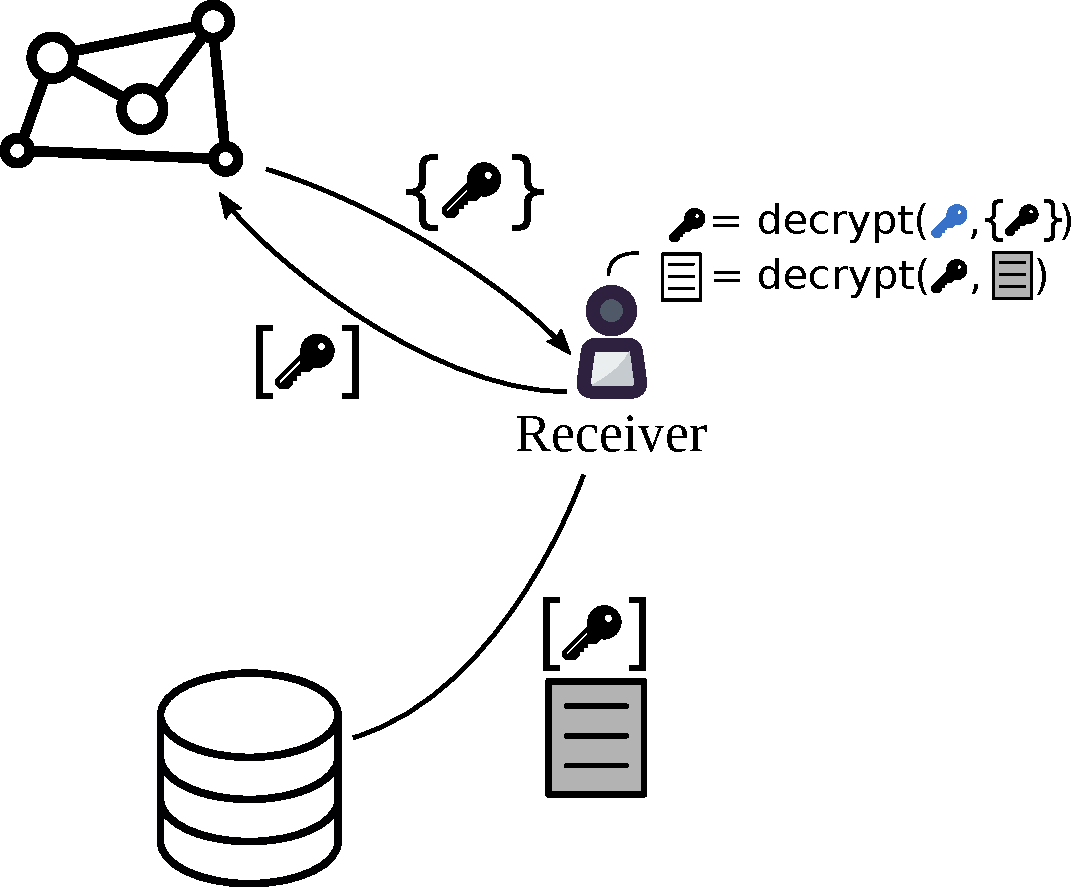
\includegraphics[height=4.5cm]{pdf/pre-kms.pdf}
        \end{figure}

        Advantages
        \begin{itemize}
            \item Data not decrypted to facilitate sharing
            \item Scalable and performant
            \item Access revocation through re-encryption key deletion
            \item Secure use of data storage providers
        \end{itemize}
    \end{frame}

    \begin{frame}
        \frametitle{Centralized KMS using PRE}
        \framesubtitle{Encryption}
        \begin{figure}
            \centering
            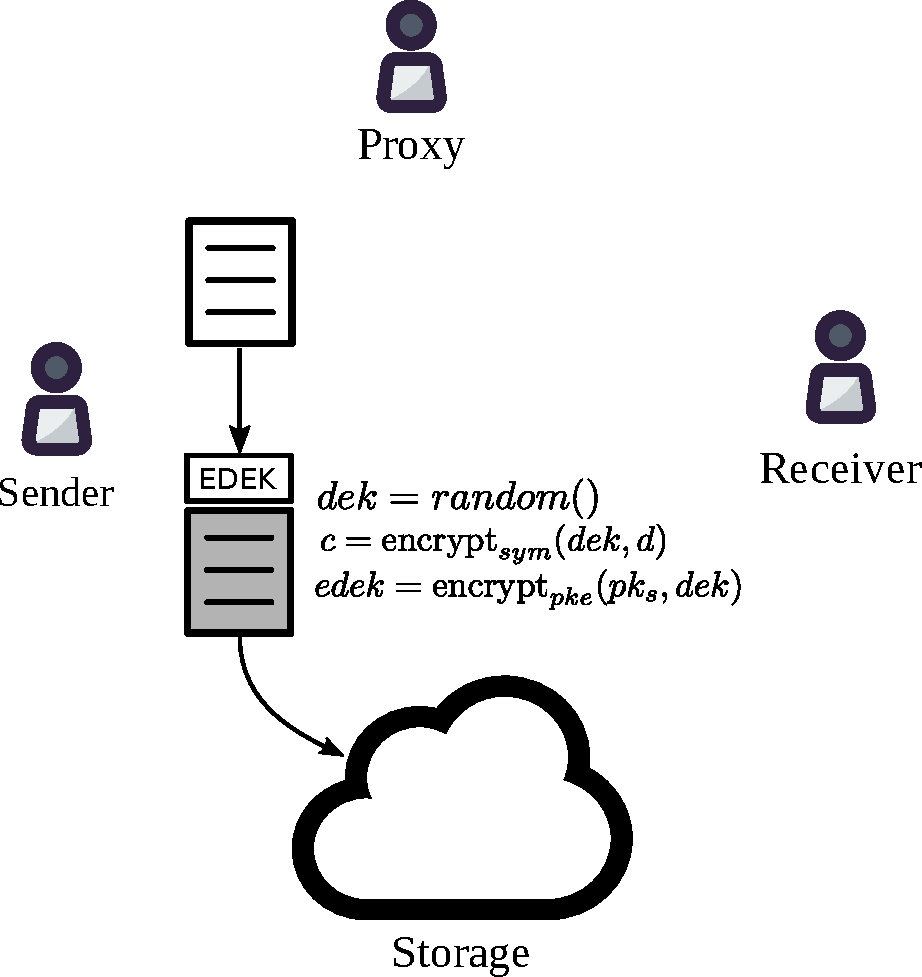
\includegraphics[height=7cm]{pdf/encrypt.pdf}
        \end{figure}
    \end{frame}

    \begin{frame}
        \frametitle{Centralized KMS using PRE}
        \framesubtitle{Access delegation}
        \begin{figure}
            \centering
            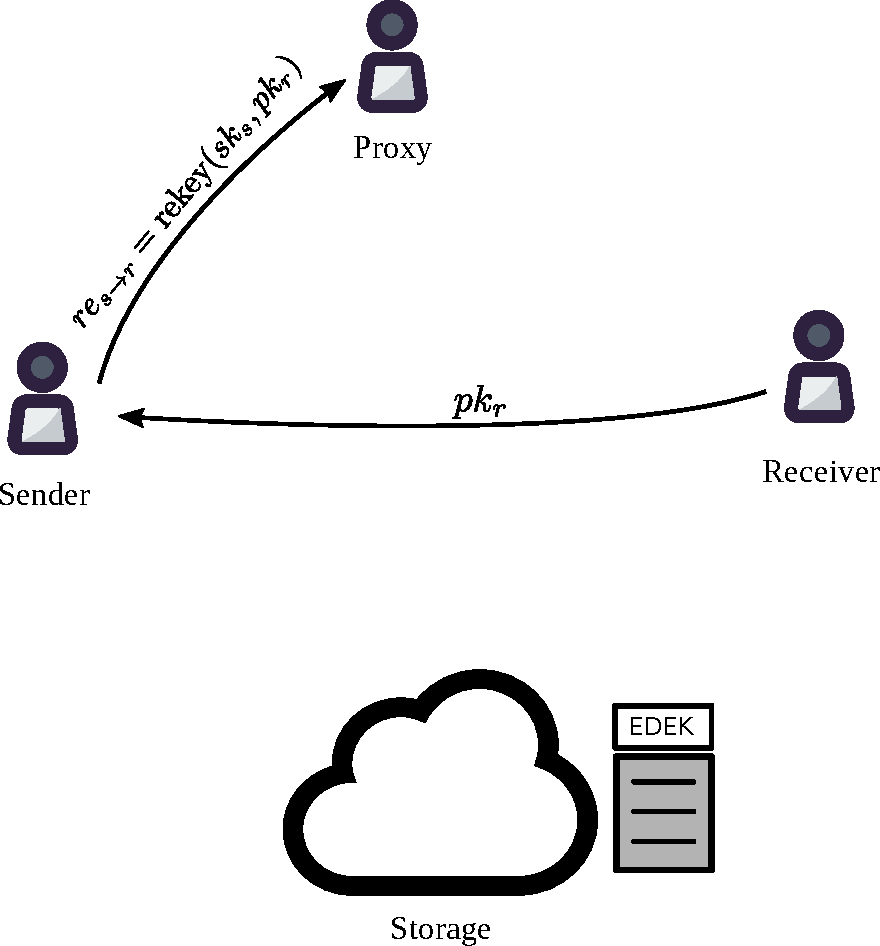
\includegraphics[height=7cm]{pdf/delegate.pdf}
        \end{figure}
    \end{frame}

    \begin{frame}
        \frametitle{Centralized KMS using PRE}
        \framesubtitle{Decryption}
        \begin{figure}
            \centering
            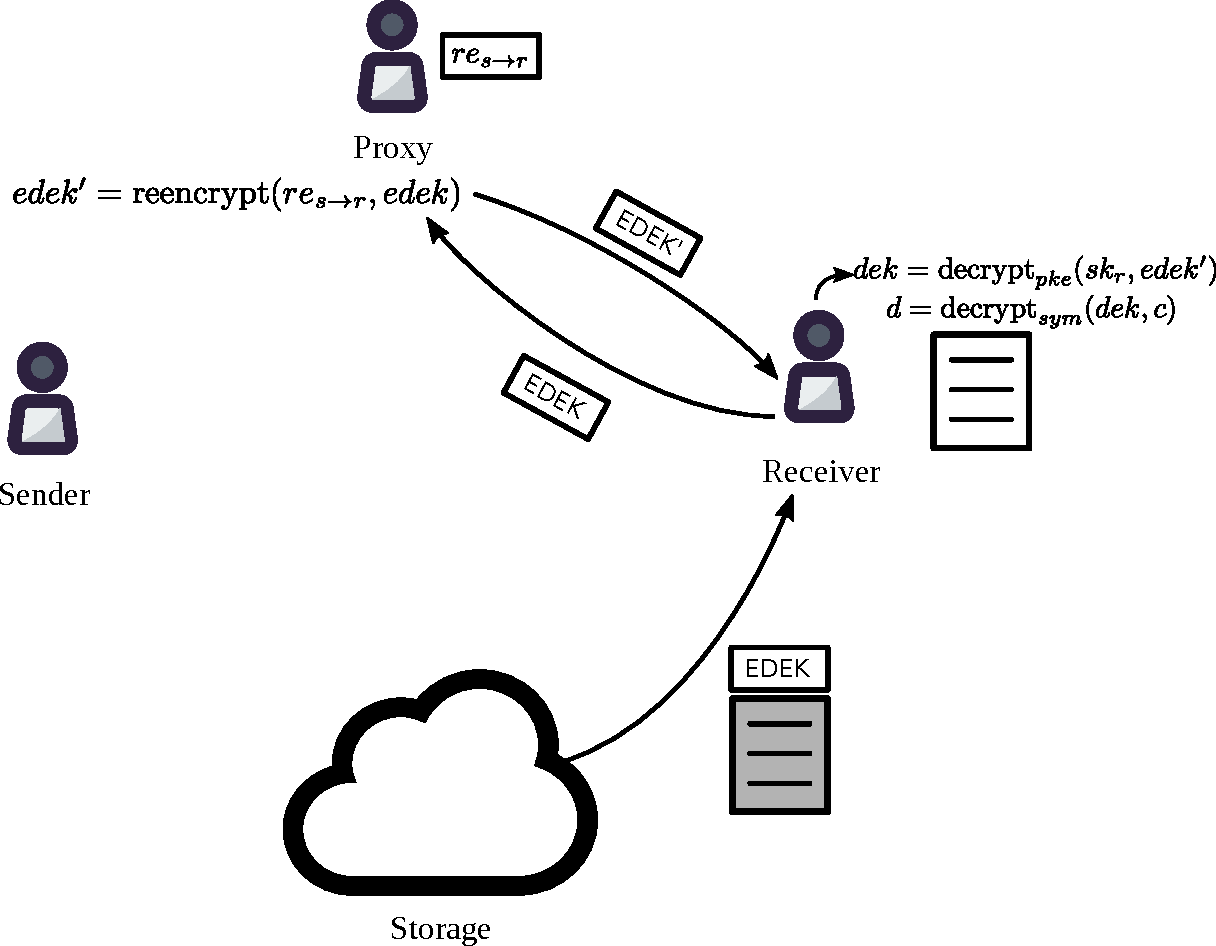
\includegraphics[height=7cm]{pdf/decrypt.pdf}
        \end{figure}
    \end{frame}

    \begin{frame}
        \frametitle{Decentralized Key Management}
        \framesubtitle{Using threshold split-key re-encryption (Umbral)}
        \begin{figure}
            \centering
            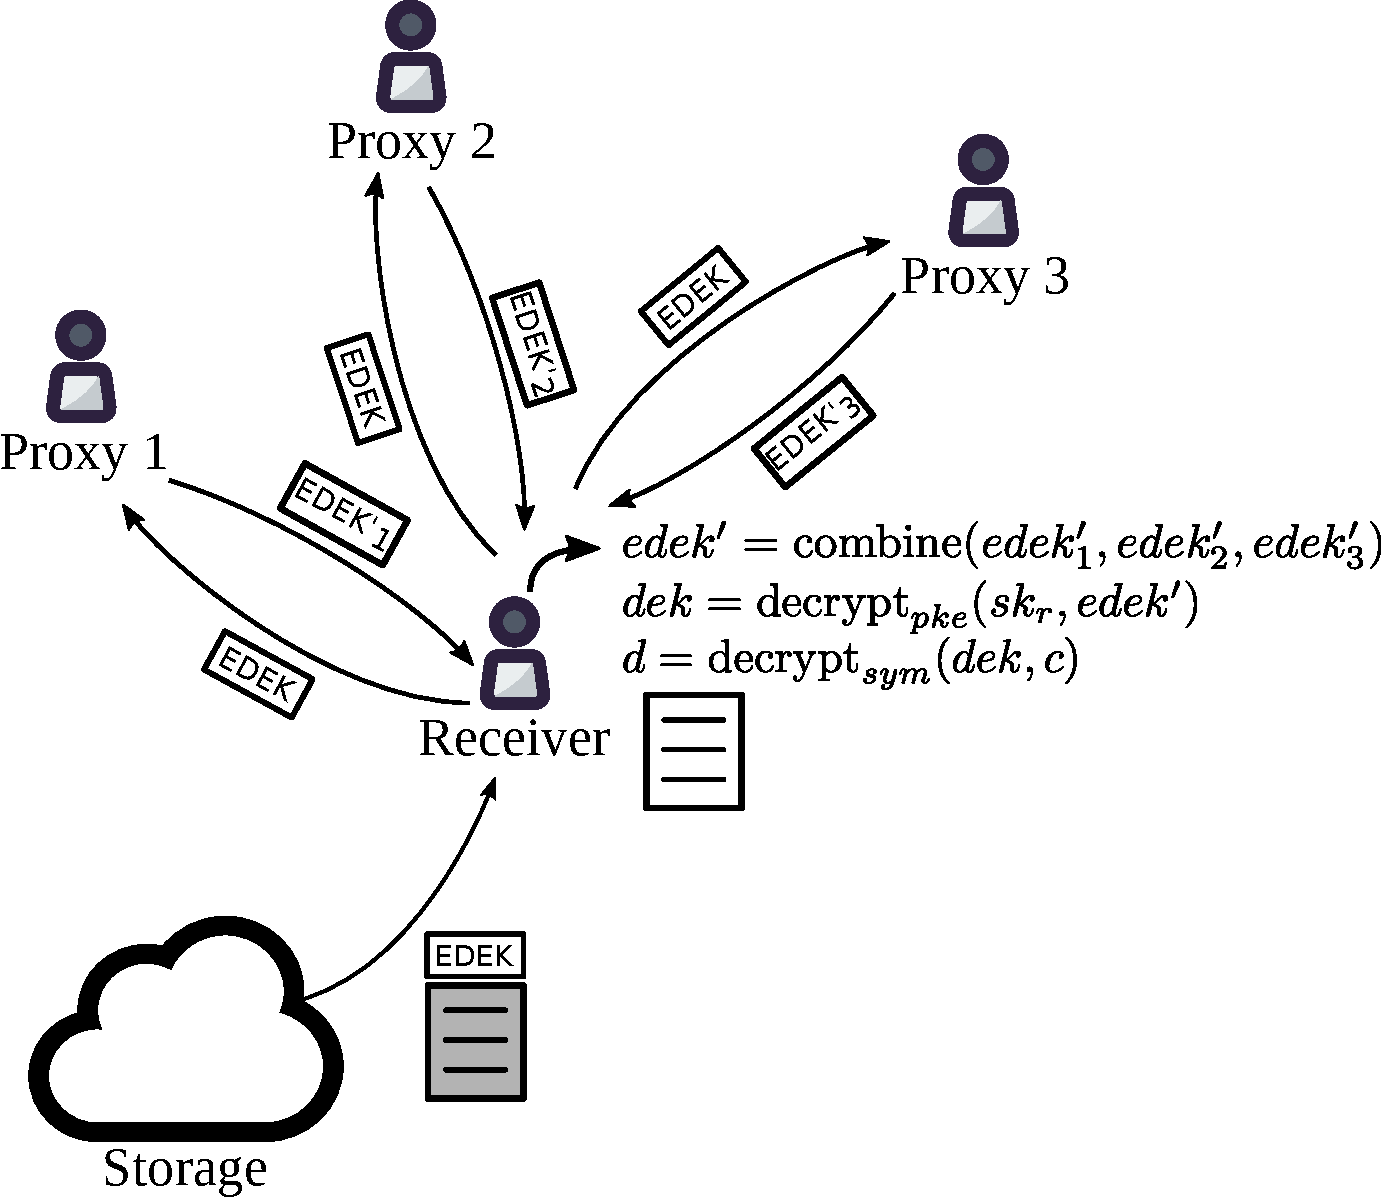
\includegraphics[height=6.5cm]{pdf/decrypt-umbral.pdf}
        \end{figure}
    \end{frame}

    \begin{frame}
        \frametitle{Umbral: Threshold Proxy Re-encryption}
        \begin{itemize}
        	\item \emph{``Umbral''} is Spanish for \emph{``threshold''}
            \item PRE properties: Unidirectional, single-hop, non-interactive
            \item Follows a KEM/DEM approach:
            	\begin{itemize}
		    \item UmbralKEM provides the threshold re-encryption capability
                    \item Uses ECIES for key encapsulation with ZK proofs of correctness for verifiability on prime order curves (such as secp256k1)
            	    \item DEM can be any authenticated encryption (currently ChaCha20-Poly1305)
        	\end{itemize}
	    \item IND-PRE-CCA security
            \item Key splitting is analogous to Shamir Secret Sharing
	    \item Verification of re-encryption correctness through Non-Interactive ZK Proofs
            \item Reference implementation: \url{https://github.com/nucypher/pyUmbral}
	    \item Documentation: \url{https://github.com/nucypher/umbral-doc}
        \end{itemize}
    \end{frame}

    \begin{frame}
        \frametitle{KMS Network: Data Sharing + Threshold PRE (Umbral)}
        \begin{figure}
            \centering
            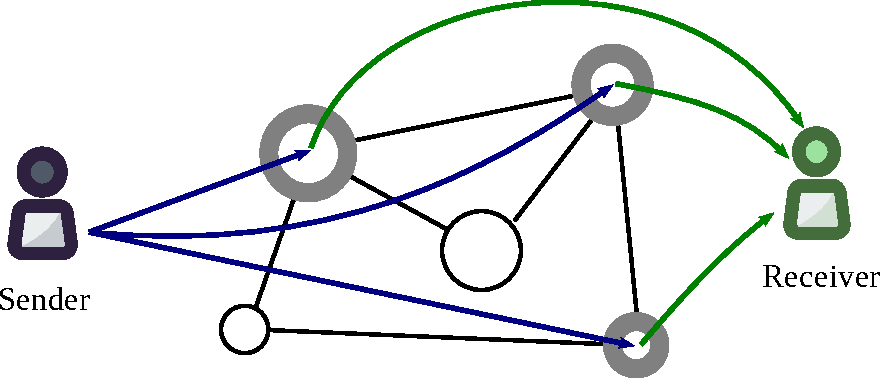
\includegraphics[height=5.5cm]{pdf/umbralnodes.pdf}
        \end{figure}
        \begin{itemize}
            \item Collusion requires $m$ nodes + receiver
        \end{itemize}
    \end{frame}

   \begin{frame}
        \frametitle{Data Sharing Policies}
        \begin{itemize}
            \setlength\itemsep{1em}
            \item Time-based
            \item Conditional on payment 
            \begin{itemize}
              \item ``Grant access once paid, continue granting while paying''
            \end{itemize}
            \item Smart contract (public) method
        \end{itemize}
        \bigskip
        Decentralized re-encryption nodes (Ursulas) relied on to apply conditions without having the ability to decrypt data
    \end{frame}

    \begin{frame}
      \frametitle{MOBI Grand Challenge}
      \framesubtitle{OBDX - Vehicle Onboard Diagnostics (OBD) Data Exchange}
      \begin{itemize}
        \item Vehicle owner securely shares OBD data with Insurance company
        \item Submission: \url{https://devpost.com/software/obdx}
        \item GitHub: \url{https://github.com/nucypher/vehicle-data-exchange}
      \end{itemize}
      \begin{figure}
        \centering
        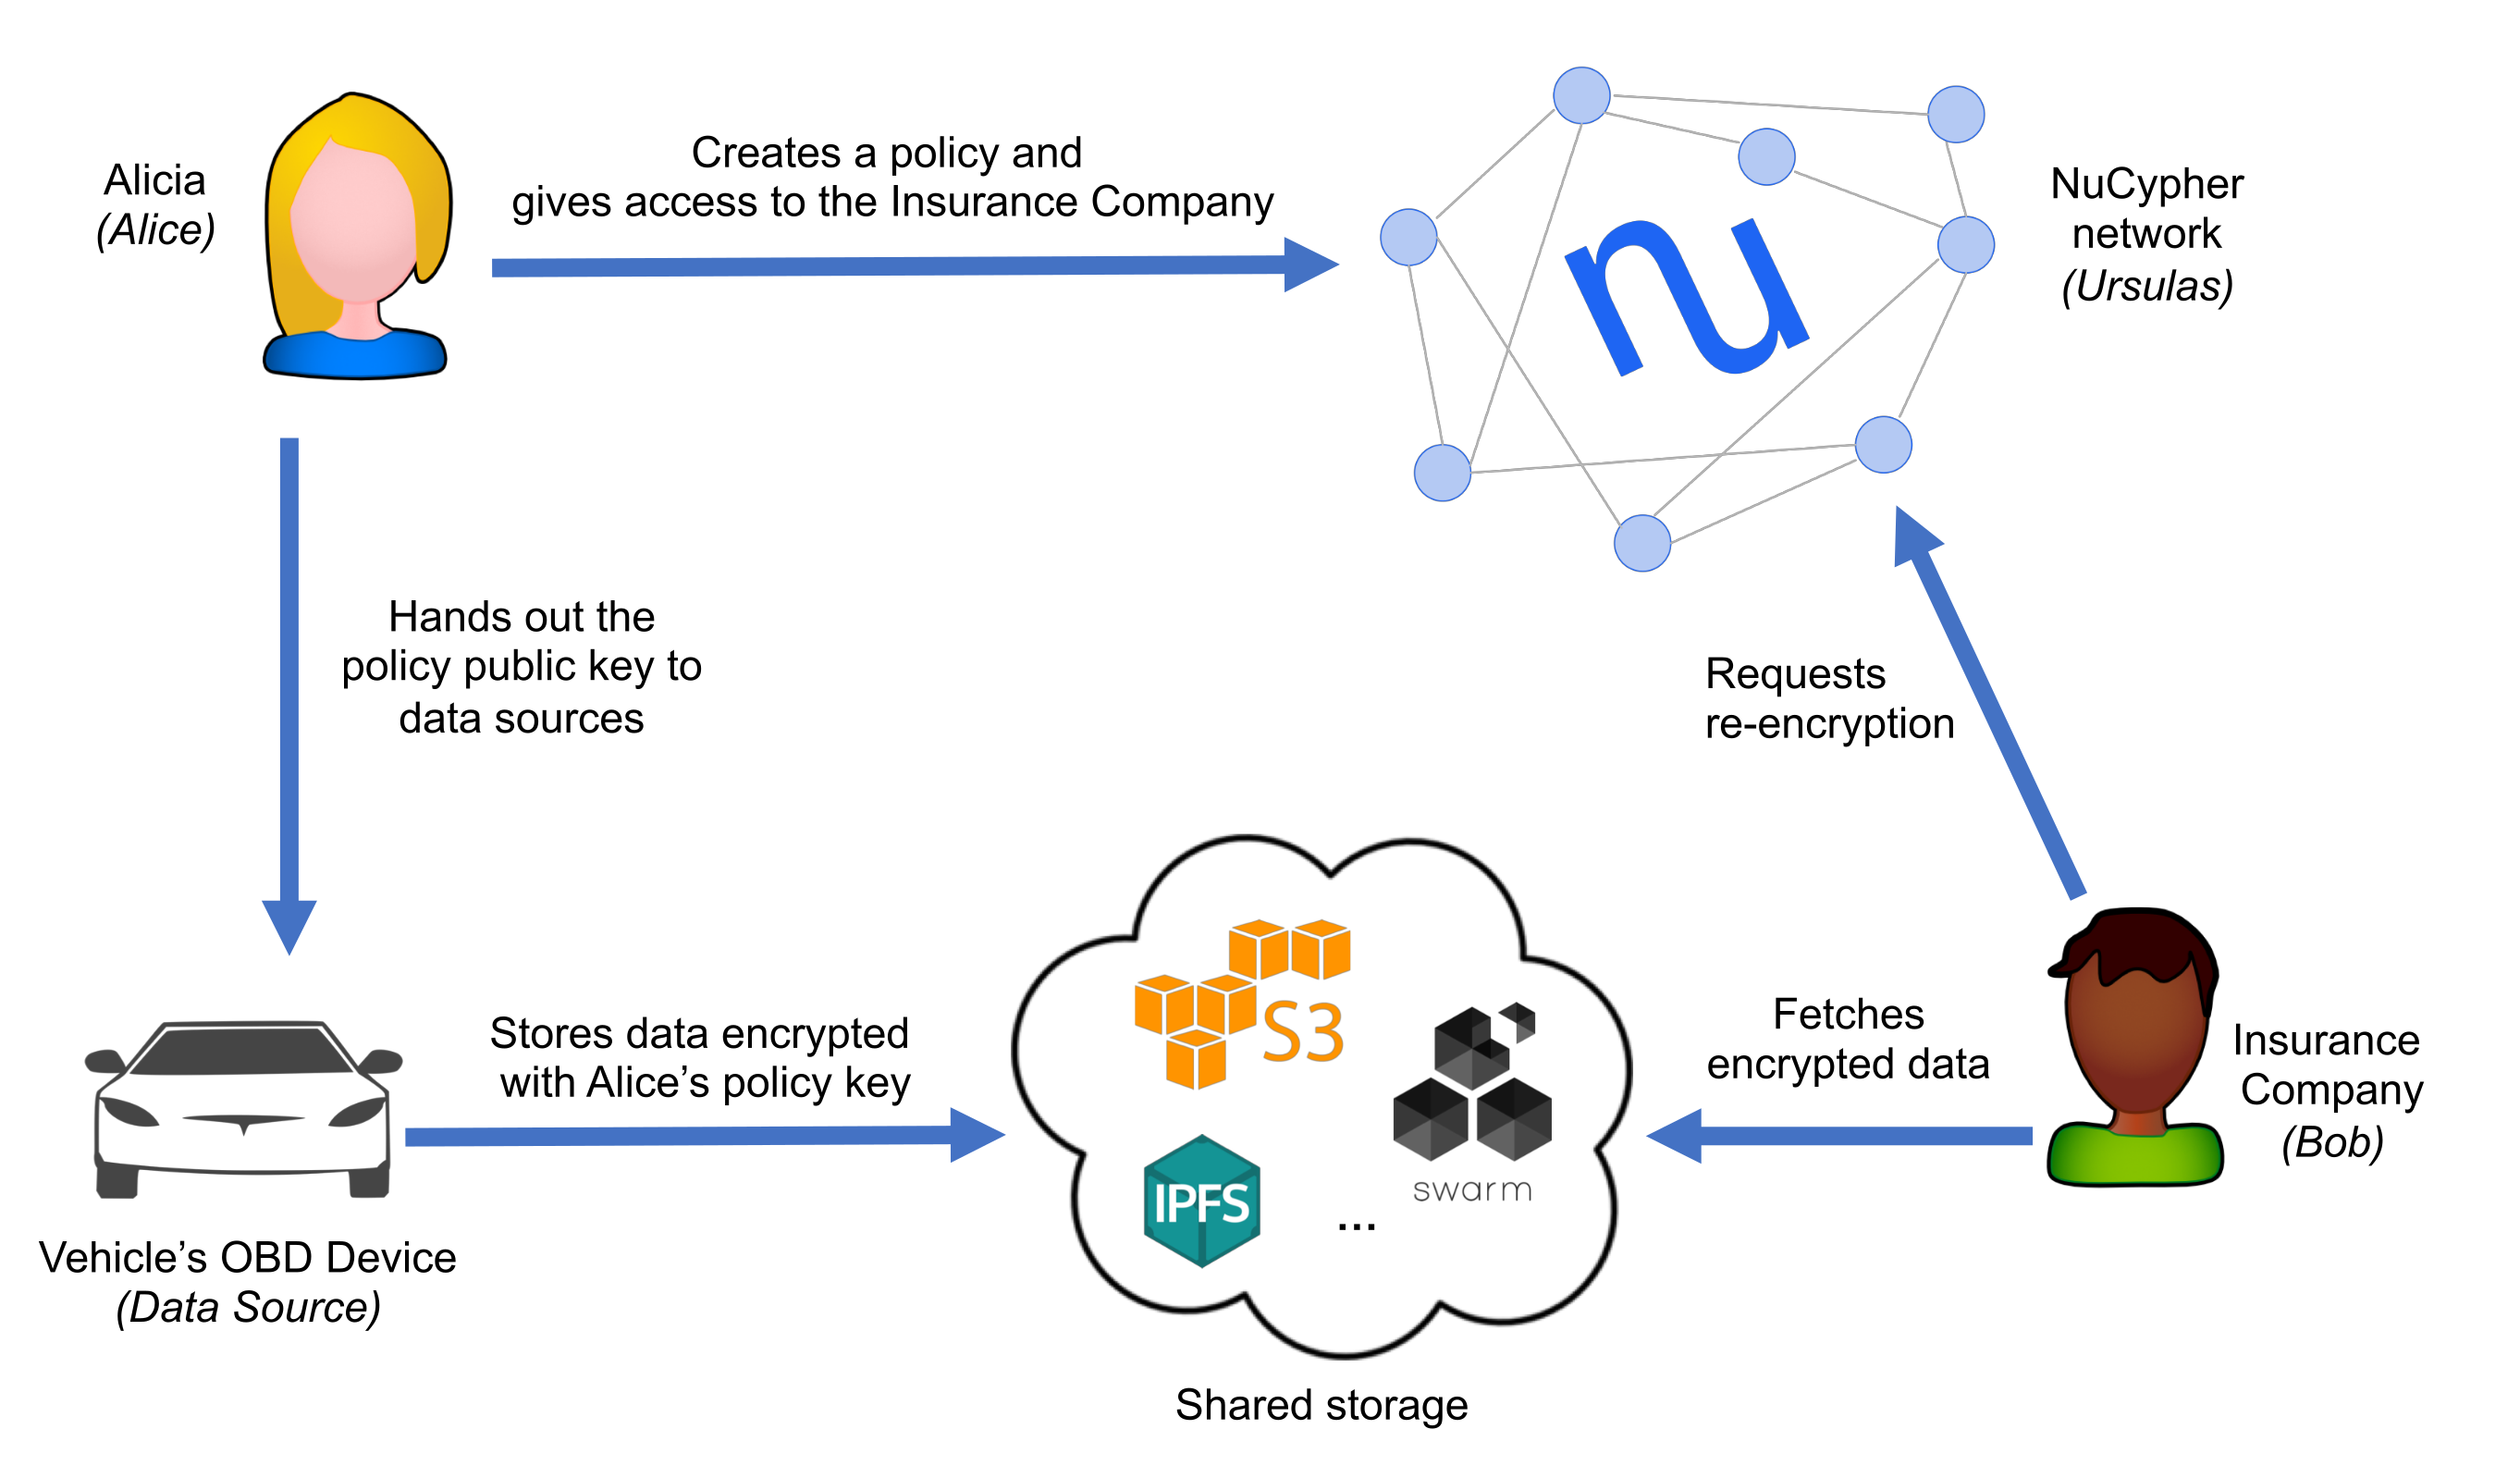
\includegraphics[height=5.5cm]{pdf/vehicle-data-exchange.png}
      \end{figure}
    \end{frame}

    \begin{frame}
      \frametitle{Demo}
      \begin{figure}
        \centering
        
\includegraphics[height=5.5cm]{pdf/terminal.pdf}
      \end{figure}
    \end{frame}

    \begin{frame}
      \frametitle{Open Questions}
      \framesubtitle{Proposed Vehicle Identity}
    \end{frame}

    \begin{frame}
      \frametitle{Early Users}
      \begin{figure}
           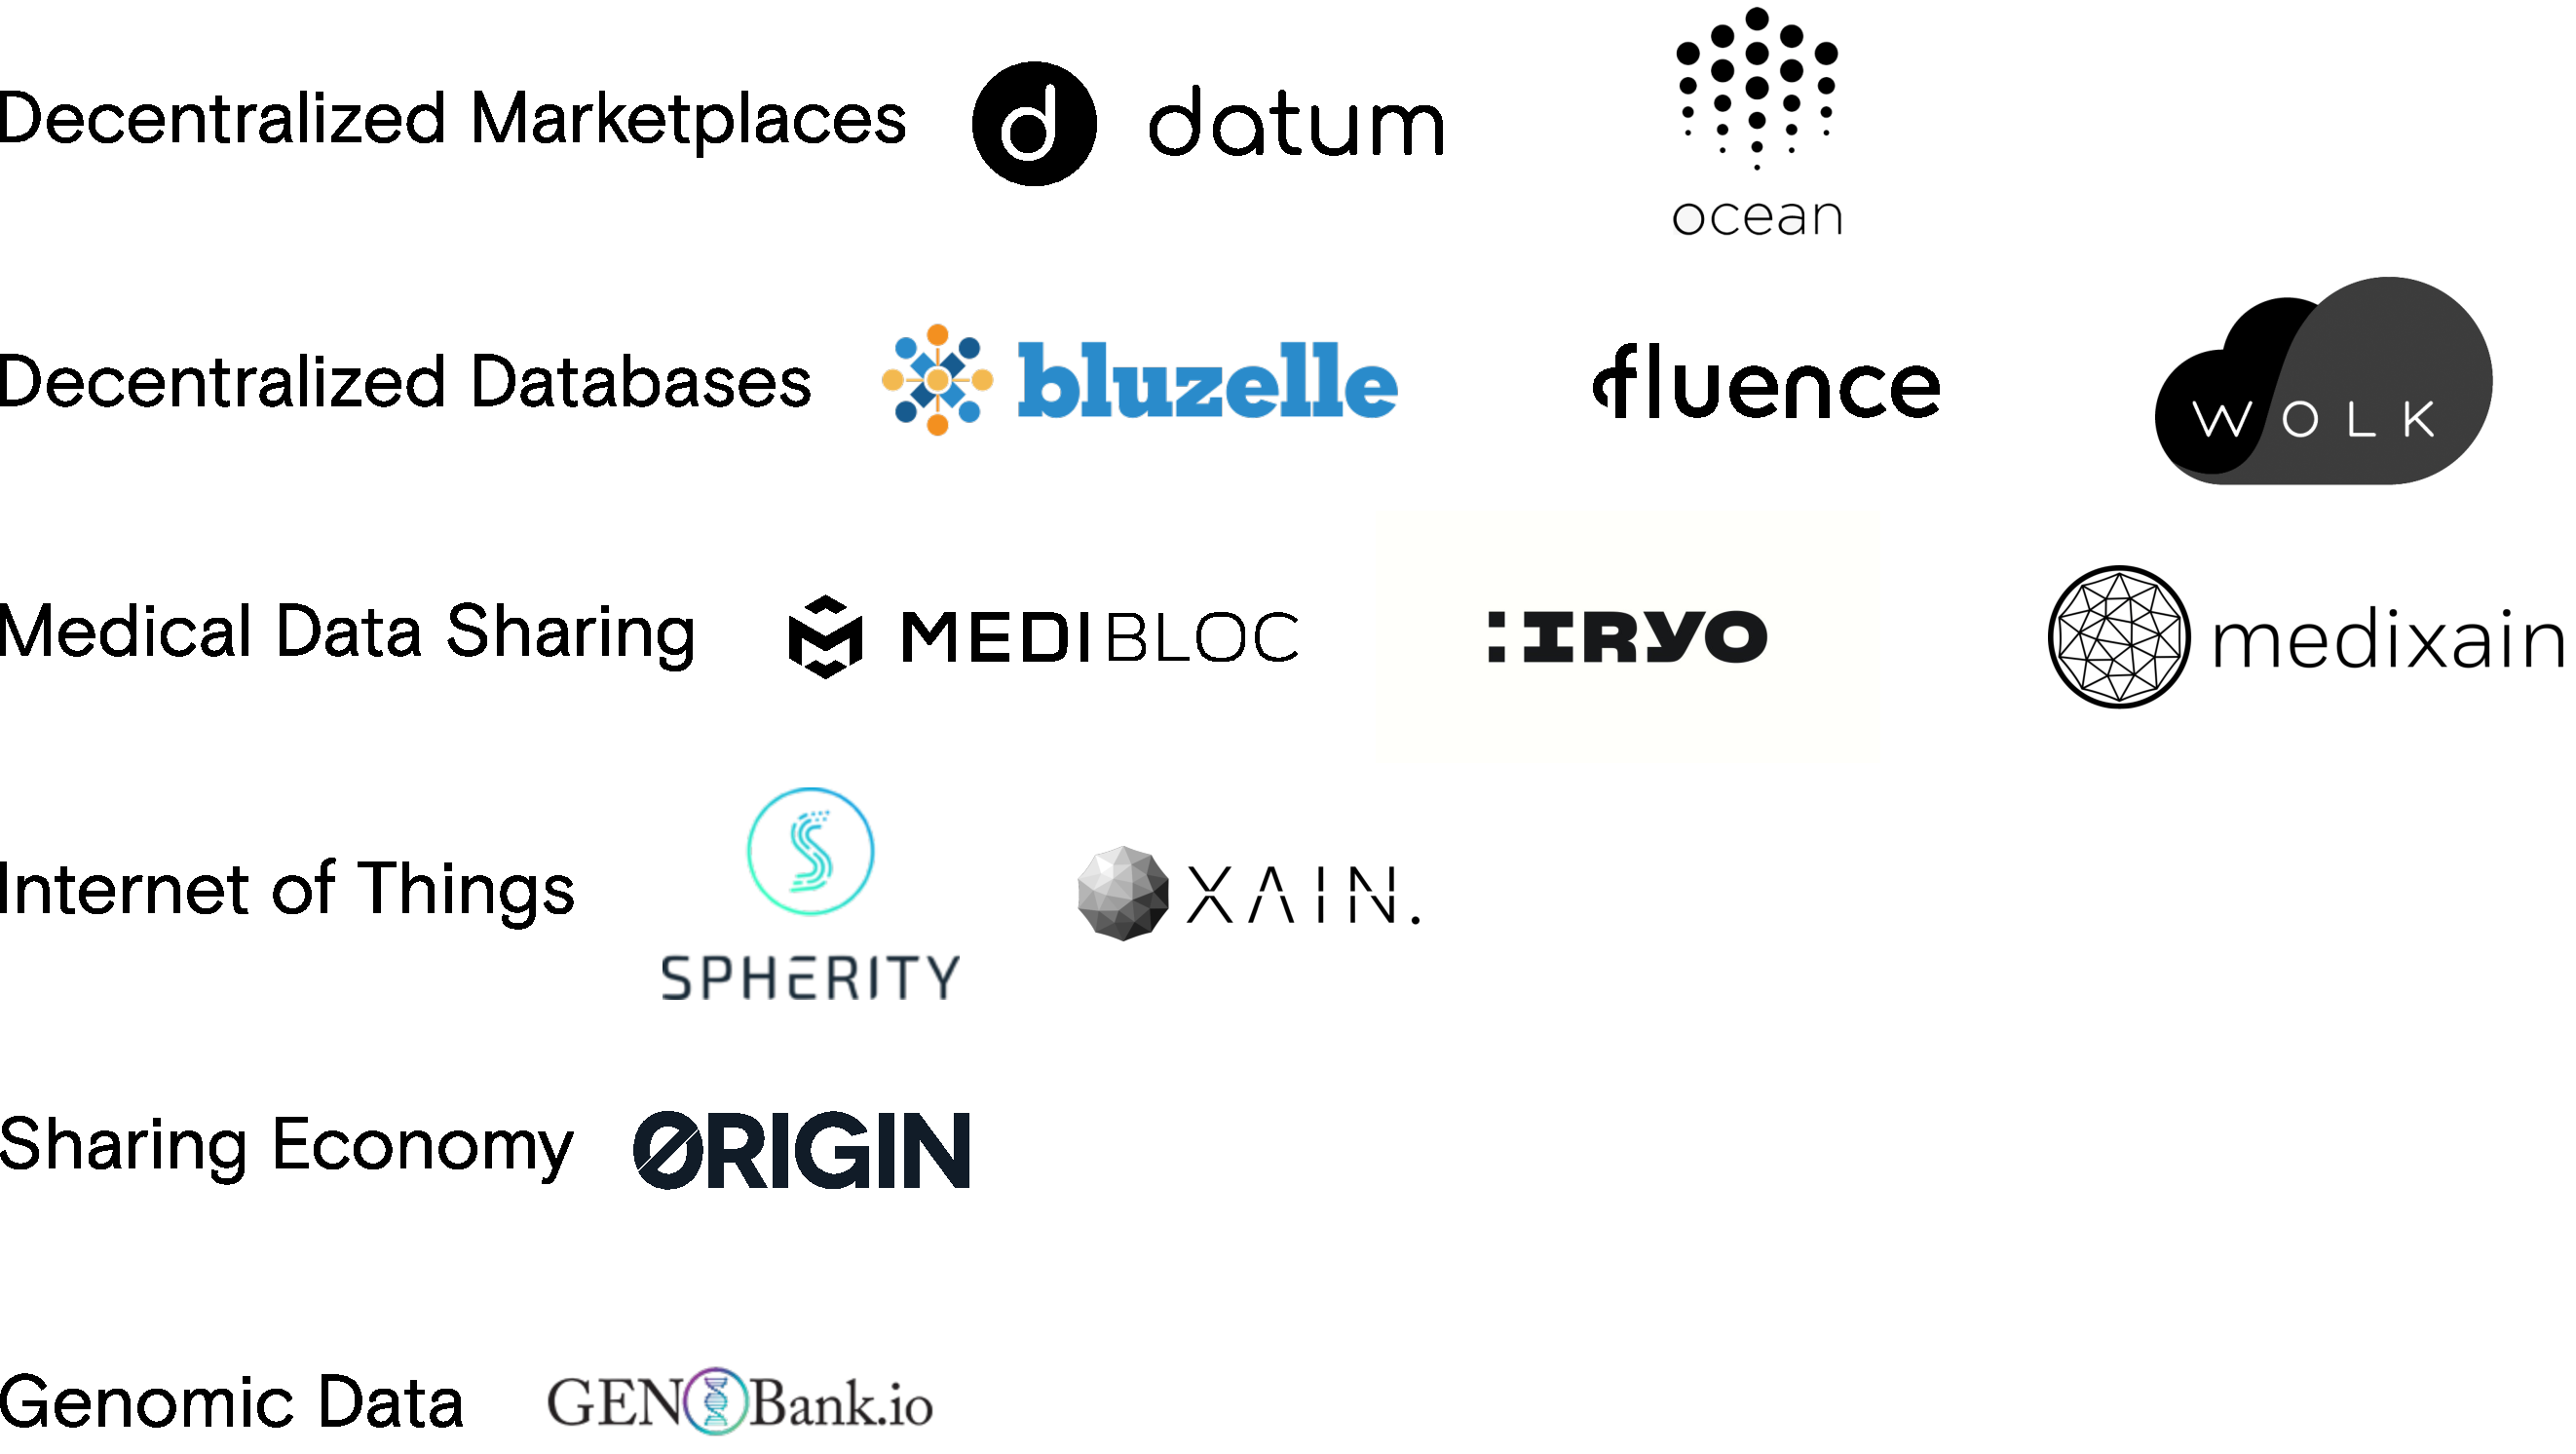
\includegraphics[width=11.5cm]{pdf/projects.pdf}
      \end{figure}
    \end{frame}

    \begin{frame}
        \frametitle{More Information}
        \begin{figure}
            \centering
            
\includegraphics[width=3cm]{pdf/nucypher_logo.pdf}
        \end{figure}
        Website: \url{https://www.nucypher.com}

        Whitepaper: \url{https://www.nucypher.com/whitepapers/english.pdf}

        Proxy Re-encryption Network: \url{https://github.com/nucypher/nucypher}

        Umbral Reference Implementation: \url{https://github.com/nucypher/pyUmbral}

        Discord: \url{https://discord.gg/7rmXa3S}

        E-mail: \href{mailto:\emailname @nucypher.com}{\emailname @nucypher.com}

        E-mail: \href{mailto:hello@nucypher.com}{hello@nucypher.com}
    \end{frame}

    \begin{frame}
      \frametitle{Appendix: Umbral Flow Diagram}
      \begin{figure}
        \centering
        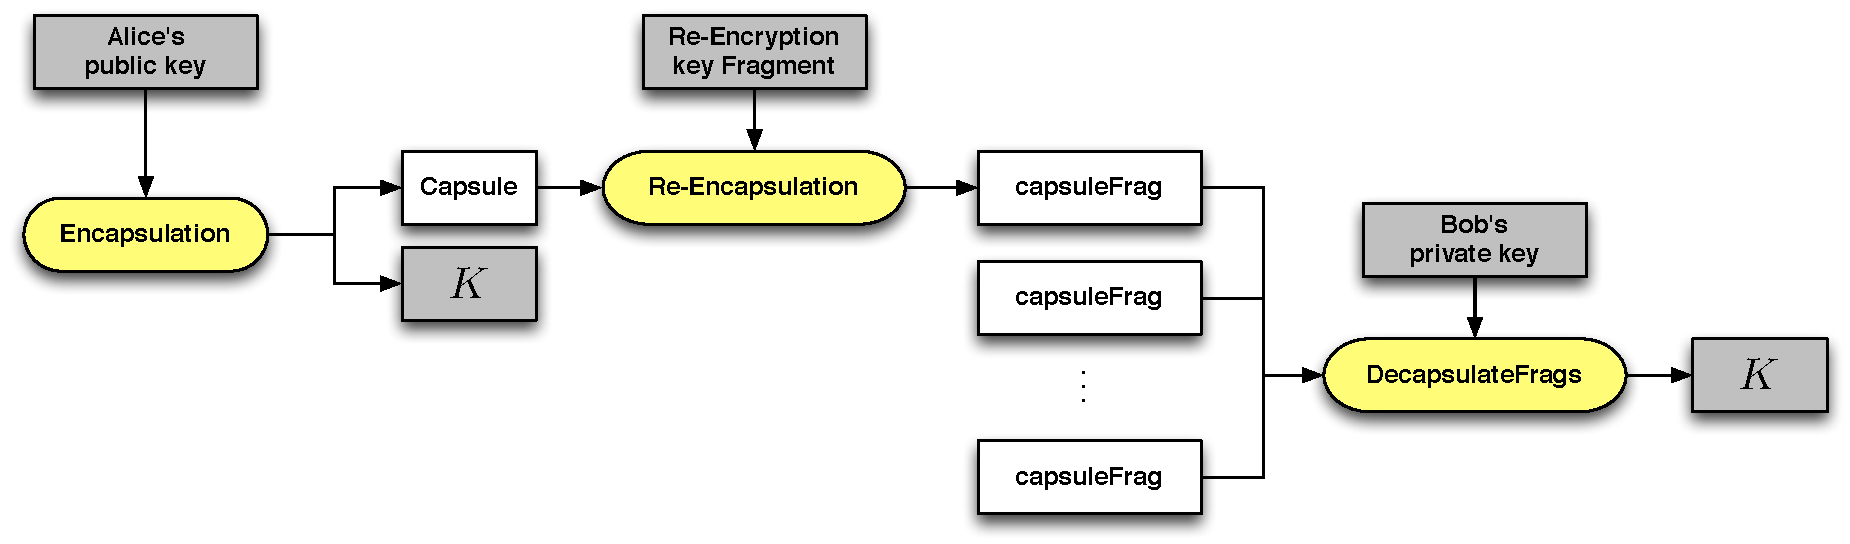
\includegraphics[width=11cm]{pdf/umbral-kem-flow.pdf}
      \end{figure}
      \begin{itemize}
           \item Reference implementation: \url{https://github.com/nucypher/pyUmbral}
           \item Documentation: \url{https://github.com/nucypher/umbral-doc}
      \end{itemize}
    \end{frame}

    \begin{frame}
        \frametitle{Appendix: Security Audits}
        \begin{figure}
            \centering
            
\includegraphics[height=2.5cm]{pdf/security-audits.pdf}
      \end{figure}
    \end{frame}

    \begin{frame}
      \frametitle{Appendix: Team}
        \begin{figure}
            \centering
            \includegraphics[width=15cm]{pdf/company.pdf}
        \end{figure}
    \end{frame}

    \begin{frame}
      \frametitle{Appendix: Investors}
        \framesubtitle{>\$15M in Venture Funding}
        \begin{figure}
            \centering
            
\includegraphics[height=6.5cm]{pdf/investors.pdf}
        \end{figure}
    \end{frame}

\end{document}

